 \documentclass[addpoints]{exam}
\usepackage{url}
\usepackage{amsmath,amsthm,enumitem}
\usepackage{amssymb}
\usepackage{graphicx}
\usepackage{xcolor}
\usepackage{algpseudocode}
\usepackage{algorithm}
\usepackage{units}
%\input myfonts

\newtheorem*{claim}{Claim}
\title{CS 6150 - Fall 2025 - HW2\\Greedy algorithms, Local search, Graph traversal \& shortest paths}
\date{Submission date:  Friday, Oct 31, 2025 (11:59 PM)}

% \def\mysolution#1{#1} % Uncomment this to reveal answers
\def\mysolution#1{}    % Uncomment this to hide answers 

\begin{document}
\maketitle
\begin{center}
\fbox{\fbox{\parbox{5.5in}{\centering
This assignment has \numquestions\ questions, for a total of \numpoints\
points. You will still be graded out of 100, and any points you earn above 100 will count as bonus and can compensate for a low score on other homeworks.
Unless otherwise specified, complete and reasoned arguments will be expected for all answers. }}}
\end{center}

\qformat{Question \thequestion: \thequestiontitle\dotfill \textbf{[\totalpoints]}}
\pointname{}
\bonuspointname{}
\pointformat{[\bfseries\thepoints]}


\begin{center}
  \gradetable
\end{center}
\newpage

{\setlength{\parindent}{0cm} \textbf{Note: Unless otherwise specified, complete and well-reasoned arguments for correctness and running time are expected for all answers. For the problems based on graphs, the different graph algorithms we covered in class (breadth-first/depth-first traversal, Dijkstra, Bellman-Ford, etc.) can be used as black-boxes if you apply them directly as we learned them. However, if you modify them to suit a given problem, spell out the modifications clearly (i.e. they are no longer black-boxes) with their effect on correctness and running time. Assume that, by default, $n$ represents the number of vertices while $m$ represents the number of edges in a graph.}}\\\\

\begin{questions}
\titledquestion{Santa's tradeoffs}[15]
Recall the matching problem we saw in class: there are $n$ gifts, and $n$ children,
and each child has a non-negative valuation for each gift. Formally, the value of
gift $j$ to child $i$ is given by $V_{i,j}$. We assume that all $V_{i,j} \ge 0$.
Santa's goal is to give one gift to each child, so as to maximize the {\em total
value} (of course, a gift cannot be given to more than one child).
Suppose we now perform a more elaborate local search, this time picking every {\em
triple} of edges in the current solution, and seeing if there is a reassignment of
gifts between the end points of these edges that can improve the total value. Prove
that a locally optimal solution produced this way has a value that is at least two-thirds ($\nicefrac{2}{3}$) of the optimum value. [This kind of trade-off is typical in local search --
each iteration is now more expensive ($O(n^3)$ instead of $O(n^2)$), but the
approximation ratio is better.]\\


\mysolution{
    \input{Sol-1}
}



\titledquestion{$t$ farthest elements from each other}
A common problem in returning search results is to display results that are {\em diverse}. A simplified formulation of the problem is as follows. We have $n$ points in Euclidean space of $d$-dimensions, and suppose that by distance, we mean the standard Euclidean distance. The goal is to pick a subset of $t$ (out of the $n$) points, so as to maximize the sum of the pairwise distances between the chosen points. 
I.e., if the points are denoted $P = \{p_1, p_2, \dots, p_n\}$, then we wish to choose an $S \subseteq P$, such that $|S| = t$, and $\sum_{p_i, p_j \in S} d(p_i, p_j)$ is maximized.

A common heuristic for this problem is local search. Start with some subset of the points, call them $S = \{q_1, q_2, \dots, q_t\} \subseteq P$. At each step, we check if replacing \underline{one of the $q_i$} with a point in $P \setminus S$ improves the objective value.  If so, we perform the swap, and continue doing so as long as the objective improves. The procedure stops when no improvement (of this form) is possible. Suppose the algorithm ends with $S = \{q_1, \dots, q_t\}$.  We wish to compare the objective value of this solution with the optimum one. Let $\{x_1, x_2, \dots, x_t\}$ be the optimum subset. 

\begin{parts}
\part[5]  Use local optimality to argue that:
\[ d(x_1, q_2) + d(x_1, q_3) + \dots + d(x_1, q_t) \le d(q_1, q_2) + d(q_1, q_3) + \dots + d(q_1, q_t). \]
\mysolution{
\input{Sol-2a}
}

\part[8] Deduce that:  [{\em Hint:} Use two inequalities of the form above.]
\[ (t-1) \cdot d(x_1, x_2) \le 2 \left[ d(q_1, q_2) + d(q_1, q_3) + \dots + d(q_1, q_t) \right]. \]
\mysolution{
\input{Sol-2b}
}

\part[10] Use this expression to argue that 
\[ \sum_{i,j} d(x_i, x_j) \le 2 \sum_{i,j} d(q_i, q_j).\]
Note: this shows that the local optimum has an objective value at least $\nicefrac{1}{2}$ the global optimum.
\mysolution{
\input{Sol-2c}
}
\end{parts}
\newpage
\titledquestion{Set Cover Revisited}
In class, we saw the set cover problem (phrased as picking the smallest set of people who cover a given set of skills). Formally, we have $n$ people, and each person has a subset of $m$ skills. Let the set of skills of the $i$th person be denoted by $S_i$, which is a subset of $[m]$ (shorthand for $\{1, 2, \dots, m\}$). 
\begin{parts}
\part[8] Suppose that there is a set of seven (7) people whose skill sets optimally cover all of $[m]$ (i.e., together, they possess all the skills). Now, suppose we run the greedy algorithm discussed in class until the set of people chosen covers at least $75\%$ of the skills. How many people must we pick using the greedy algorithm to ensure this coverage?

\textbf{In class we proved the following theorem}

\textbf{Suppose there is an optimum solution that uses $k$ people. Then the greddy algorihtm does not use more than $k\log_{e}{m}$ people}

\mysolution{
\input{Sol-3a}
}

\part[6] Consider the following ``street surveillance'' problem. We have a graph $(V, E)$ with $n$ nodes and $m$ edges. We are allowed to place surveillance cameras at the nodes. Once placed, they can monitor all the edges incident to the node. The goal is to place as few cameras as possible, so as to monitor {\bf all the edges} in the graph. Show how to cast the street surveillance problem as Set Cover.

\mysolution{
\input{Sol-3b}
}

\part[10] Let $(V, E)$ be a graph as above, and suppose that the optimal solution for the street surveillance problem places $k$ cameras (and is able to monitor all edges).  Now consider the following ``lazy'' algorithm: 
\begin{enumerate}
\item initialize $S = \emptyset$
\item while there is an unmonitored edge $\{i,j\}$:  \\
		$~~~~~~$add both $i, j$ to $S$ and mark all their edges as monitored
\end{enumerate}
Clearly (due to the while loop), the algorithm returns a set $S$ that monitors all the edges.  Prove that the set also satisfies $|S| \le 2k$ (recall that $k$ is the number of nodes in the optimal solution).

{\sc Moral.}  Even though the algorithm looks ``dumber'' than the greedy algorithm, it has a better approximation guarantee --- $2$ versus $\log n$.
\end{parts}

{\em Hint.} Consider the edges $\{i,j\}$ encountered when we run the algorithm. Could it be that the optimal set chooses {\em neither} of $\{i,j\}$?

\mysolution{
\input{Sol-3c}
}

\titledquestion{Kruskal's MST algorithm}[10]
Here is Kruskal's greedy algorithm to find a minimum spanning tree of a weighted, undirected, connected graph $G(V_G,E_G)$, where $V_G$ is the set of vertices with $|V_G|=n$, and $E_G$ is the set of edges with $|E_G|=m$.
\begin{algorithmic}[1]
    \Function{Kruskal }{$~G(V_G,E_G)~$}
    \State Sort $E_G$ in monotonically increasing order of edge weight.
    \State Let graph $T=(V_T,E_T)$ where $V_T=V_G$ and $E_T=\emptyset$.
    
    \Comment{In other words, $T$ has all vertices of $G$, but no edges.}
    \For {edge $u$---$v$ in sorted $E_G$}
        \If{$u$---$v$ does not complete a cycle in $T$}
            \State Add edge $u$---$v$ to $T$.
        \EndIf
    \EndFor
    \State \Return $T$
    \EndFunction
\end{algorithmic}

Prove that, even though the for-loop at line 4 runs over all edges of $G$, \textsc{Kruskal} adds exactly $n-1$ edges to $T$. [Hint: \textit{Think about the number of disconnected components in $T$.}]
\mysolution{
\input{Sol-4a}
}

\titledquestion{Let's plan a road trip}[15]
Imagine you are planning a long road trip from your home $h$ to your destination $d$. You have a roadmap in the form as a \textbf{simple, weighted, undirected graph} $G(V,E)$, and you need to plan your journey using it. Your trip is going to take several days, and there are a few vertices in the graph that have hotels where you can spend the night. Let $H$ be the set of vertices with hotels, and $H \subset V-\{h,d\}$. The edge weights (represented as $t_{pq}$ for edge $p$---$q$) are positive integers indicating the \textbf{number of hours} required to travel along the edge. E.g. the figure below represents one such graph, where $H=\{b,c,i\}$ and $t_{ha}=3$, $t_{ab}=5$, and so on.

\begin{figure}[h!]
    \centering
    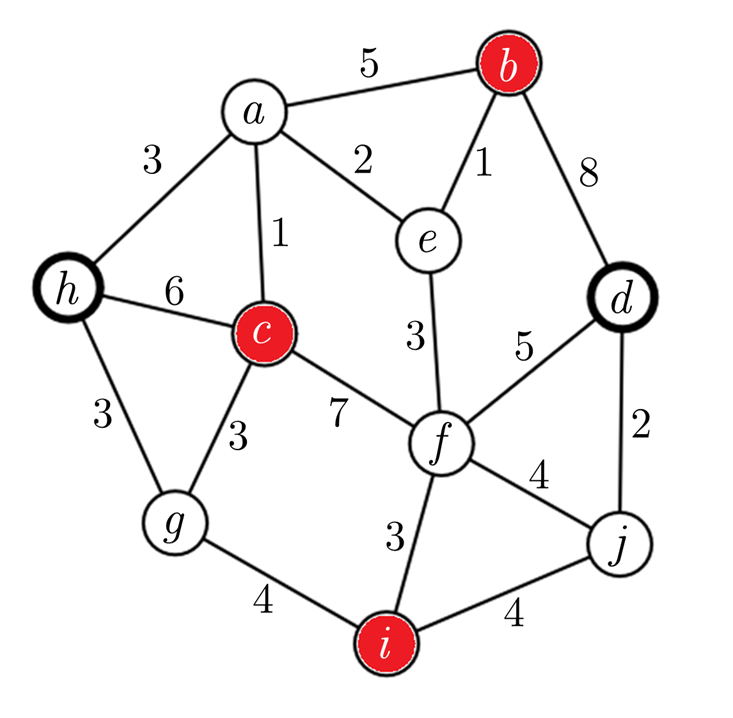
\includegraphics[width=0.35\linewidth]{hotels.png}
\end{figure}

You can spend a maximum of 7 hours each day driving. After traveling \textbf{at most} 7 hours, you must reach a hotel to sleep. From that vertex, you can start driving for another 7 hours the next day. Given a graph $G(V,E)$ and the subset $H$, give a \textbf{polynomial-time} (in $m$ and $n$) algorithm that finds out if it is possible to reach $d$ (starting from $h$) under the 7-hours-per-day constraint. There is no limit on how many days you take. E.g. in the graph shown above, it is possible to travel from $h$ to $d$ under the given constraints using many possible paths, such as $h-g-\textcolor{red}{i}-j-d$ (2 days), or $h-a-e-\textcolor{red}{b}-e-f-\textcolor{red}{i}-j-d$ (3 days). Your algorithm only needs to return yes or no (possibility of reaching $d$), and outputting the number of days and the exact path is not necessary.

It is okay if you do not include a formal proof of correctness. Please give: i) a brief description of your problem-solving approach, ii) the pseudocode, and iii) analysis of the running time. 

\mysolution{
\input{Sol-5}
}

\titledquestion{All-Pairs Shortest Paths (APSP)}
Given a directed graph $G = (V, E)$ with non-negative edge lengths $\{w_e\}$, we define the {\em distance matrix} $M$ as the $n \times n$ matrix ($n = |V|$ as usual) whose $i,j$'th entry is the shortest path distance between vertices $i$ and $j$. Given the graph (vertices, edges and lengths), the goal of the APSP problem is to find the matrix $M$.

In what follows, let $G$ be an {\bf unweighted, undirected} graph (all edge lengths are $1$). Thus, in this case, shortest path from one vertex $u$ to the rest of the vertices can be found via a simple BFS. (Thus the APSP problem can be solved in time $O(n(m+n)) = O(n^3)$.)

Let $A$ denote the {\em adjacency matrix} of the graph, i.e., an $n \times n$ matrix whose $ij$'th entry is $1$ if $ij$ is an edge, and is $0$ otherwise.  Now, consider powers of this matrix $A^k$ (defined by traditional matrix multiplication).  Also, for convenience, define $A^0 = I$ (identity matrix of size $n\times n$). 

\begin{parts}
\part[10] Prove that for any two vertices $i,j$, their distance in the graph $d(i,j)$ is the smallest $k\ge 0$ such that $A^k (i,j) > 0$.\\

\mysolution{
\input{Sol-6a}
}

\part[8] The idea is to now use fast algorithms for computing matrix multiplications. Suppose there is an algorithm that can multiply two $n \times n$ matrices in time $O(n^{2.5})$.  Use this to prove that for any parameter $k$, in $O(k n^{2.5})$ time, we can find $d(i,j)$ for all pairs of vertices $(i,j)$ such that $d(i,j) \le k$.

\mysolution{
\input{Sol-6b}
}

In other words, we can find all the {\em small} entries of the distance matrix. Let us see a different procedure that can handle the ``big'' entries.

\part[5] Let $i,j$ be two vertices such that $d(i,j) \ge k$.  Prove that if we sample $(2 \ln n) \cdot \frac{n}{k}$ vertices of the graph uniformly at random, the probability of not sampling any vertex on the shortest path from $i$ to $j$ is $\le \frac{1}{n^2}$. [{\em Hint:} You may find the inequality $1-x \le e^{-x}$ helpful.]
\end{parts}

\mysolution{
\input{Sol-6c}
}
\end{questions}
\end{document}
